\subsection{O4: the confidence gate}
\label{sec:gateexp}
\paragraph{Labels.} A gate is judged by the restoration it guards. A case is \emph{helpful} if the
RL restoration with the estimated PSF is better than the input (PSNR on synthetic data, OCR
character accuracy on real plates) and \emph{harmful} if it is worse.

\paragraph{Signals.} Table~\ref{tab:auc} ranks the candidate signals by ROC AUC for predicting a
helpful restoration on the development sets. On synthetic data all four signals are strong
(AUC 0.91--0.97), with the proposal's dip depth the best. On real plates the picture changes:
on LPBlur dip depth and peak ratio remain informative (0.79--0.80), while on CCPD-Blur, where
only 4 of 150 restorations help at all, no single signal ranks well. The gate therefore needs a
test that targets the reason CCPD restorations fail --- the blur is not one uniform line --- which is
what split-half agreement checks.

\begin{table}[h]
\centering\small
\resizebox{\textwidth}{!}{\begin{tabular}{lcccc}
\toprule
dev set & dip depth & directional contrast & peak ratio & split-half agreement \\
\midrule
synthetic (all) & \textbf{0.97} & 0.91 & 0.94 & 0.93 \\
\quad plates & \textbf{1.00} & 0.93 & 0.99 & 0.97 \\
LPBlur & 0.79 & 0.64 & \textbf{0.80} & 0.60 \\
CCPD-Blur (4 helpful of 150) & 0.58 & 0.47 & 0.69 & 0.45 \\
\bottomrule
\end{tabular}}
\caption{ROC AUC of each gate signal for ``the restoration will help'' (text-aware estimator, dev data).}
\label{tab:auc}
\end{table}

\paragraph{Calibration.} A grid over the thresholds of dip depth, directional contrast and
agreement was scored on each development set by the \emph{net share} --- the net change the gate
lets through divided by the total change at stake, $\sum_{\text{accepted}} \Delta /
\sum |\Delta| \in [-1,1]$, so that refusing everything scores 0 and every harmful restoration is
charged at its full cost --- and the gate with the best mean over the three sets was frozen:
\[
  \text{accept} \iff \text{dip depth} \ge 4.4\,\sigma \;\wedge\; \ge 2 \text{ of the 4 image halves agree}.
\]
For comparison we also report the strictest operating point, which harms at most 5\% of the images
of every development set (dip depth $\ge 4.2\sigma$, directional contrast $\ge 4\sigma$, $\ge 3$
halves agree). Figure~\ref{fig:tradeoff} shows the full trade-off between harm avoided and helpful
restorations withheld.

\begin{figure}[h]
\centering
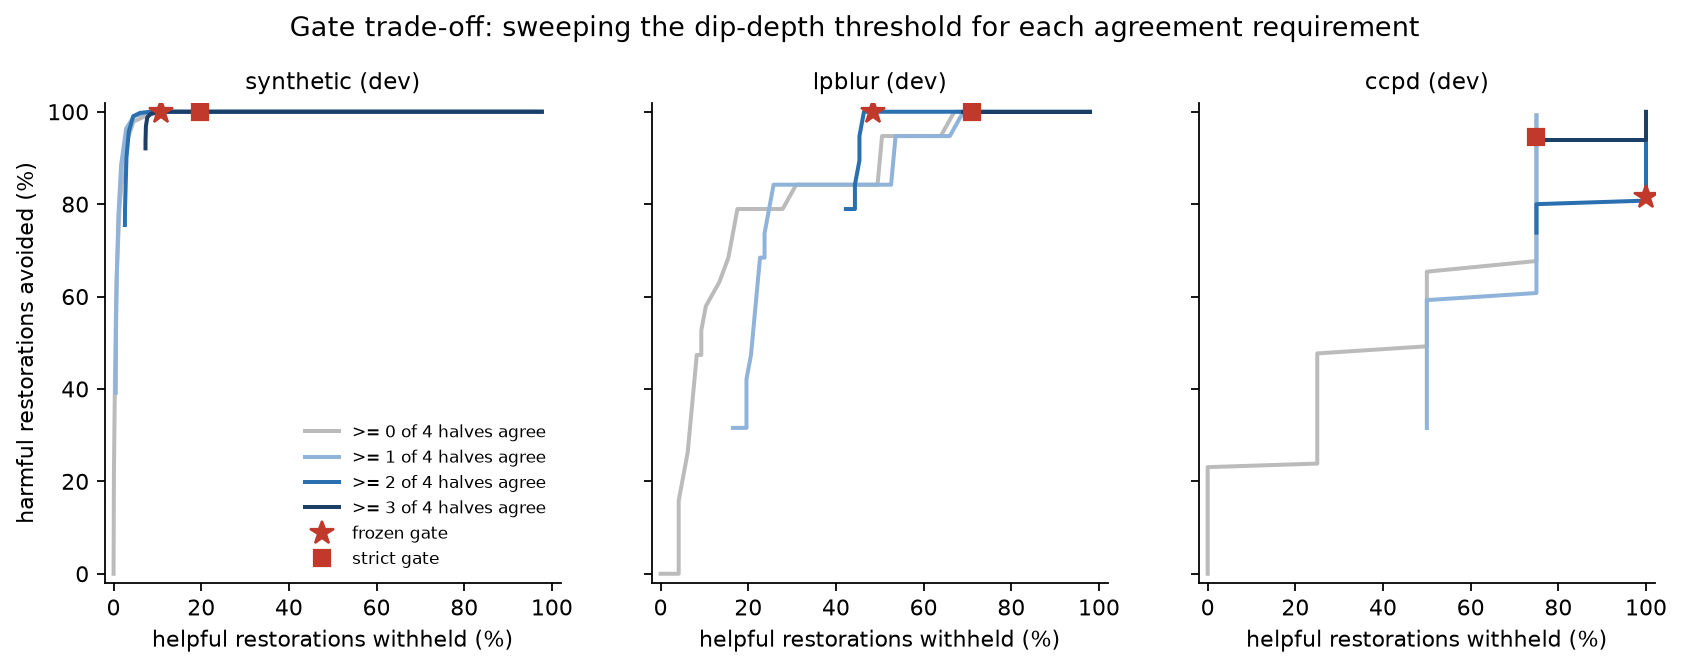
\includegraphics[width=\textwidth]{04_gate_tradeoff.png}
\caption{Harm avoided vs.\ helpful restorations withheld on the development sets, sweeping the
dip-depth threshold for each agreement requirement. CCPD-Blur has only four helpful cases, hence
the coarse steps.}
\label{fig:tradeoff}
\end{figure}

\paragraph{Held-out synthetic test.} Table~\ref{tab:gatetest} applies the frozen gate to the test
trials of Section~\ref{sec:preproc}. It refuses almost every harmful restoration (96--100\%) while
withholding 2--23\% of the helpful ones, and the share of images made worse falls from 4--20\% to
at most 0.4\%. Because the refused cases are exactly the ones with large losses, the mean PSNR gain
over all trials \emph{rises}, e.g.\ from $+1.5$ to $+3.0$\,dB on plates with the text-aware estimator.

\begin{table}[h]
\centering\small
\resizebox{\textwidth}{!}{\begin{tabular}{llcccccc}
\toprule
class & estimator & accepted & harm avoided & helpful withheld & images harmed & \multicolumn{2}{c}{mean gain (dB)} \\
 & & & & & (no gate $\rightarrow$ gate) & no gate & gate \\
\midrule
natural & baseline & 65\% & 99.7\% & 22\% & 14.8\% $\rightarrow$ 0.0\% & 0.24 & 1.25 \\
natural & text-aware & 60\% & 100\% & 23\% & 20.0\% $\rightarrow$ 0.0\% & $-0.31$ & 1.20 \\
text & baseline & 97\% & 100\% & 2\% & 0.7\% $\rightarrow$ 0.0\% & 2.14 & 2.19 \\
text & text-aware & 93\% & 100\% & 3\% & 4.1\% $\rightarrow$ 0.0\% & 1.74 & 2.12 \\
plate & baseline & 80\% & 96\% & 14\% & 7.0\% $\rightarrow$ 0.3\% & 2.34 & 3.06 \\
plate & text-aware & 78\% & 96\% & 13\% & 11.6\% $\rightarrow$ 0.4\% & 1.54 & 3.01 \\
\bottomrule
\end{tabular}}
\caption{The frozen gate on the held-out synthetic test split (2{,}560--3{,}840 trials per row).}
\label{tab:gatetest}
\end{table}
